\documentclass[a4paper]{book}
\usepackage{makeidx}
\usepackage{graphicx}
\usepackage{multicol}
\usepackage{float}
\usepackage{listings}
\usepackage{color}
\usepackage{ifthen}
\usepackage[table]{xcolor}
\usepackage{textcomp}
\usepackage{alltt}
\usepackage{ifpdf}
\ifpdf
\usepackage[pdftex,
            pagebackref=true,
            colorlinks=true,
            linkcolor=blue,
            unicode
           ]{hyperref}
\else
\usepackage[ps2pdf,
            pagebackref=true,
            colorlinks=true,
            linkcolor=blue,
            unicode
           ]{hyperref}
\usepackage{pspicture}
\fi
\usepackage[utf8]{inputenc}
\usepackage{mathptmx}
\usepackage[scaled=.90]{helvet}
\usepackage{courier}
\usepackage{sectsty}
\usepackage[titles]{tocloft}
\usepackage{doxygen}
\lstset{language=C++,inputencoding=utf8,basicstyle=\footnotesize,breaklines=true,breakatwhitespace=true,tabsize=8,numbers=left }
\makeindex
\setcounter{tocdepth}{3}
\renewcommand{\footrulewidth}{0.4pt}
\renewcommand{\familydefault}{\sfdefault}
\begin{document}
\hypersetup{pageanchor=false}
\begin{titlepage}
\vspace*{7cm}
\begin{center}
{\Large Reference Manual}\\
\vspace*{1cm}
{\large Generated by Doxygen 1.7.4}\\
\vspace*{0.5cm}
{\small Thu Apr 19 2012 08:27:30}\\
\end{center}
\end{titlepage}
\clearemptydoublepage
\pagenumbering{roman}
\tableofcontents
\clearemptydoublepage
\pagenumbering{arabic}
\hypersetup{pageanchor=true}
\chapter{Class Index}
\section{Class List}
Here are the classes, structs, unions and interfaces with brief descriptions:\begin{DoxyCompactList}
\item\contentsline{section}{\hyperlink{classBooleanExpression}{BooleanExpression} }{\pageref{classBooleanExpression}}{}
\item\contentsline{section}{\hyperlink{structEdge}{Edge} }{\pageref{structEdge}}{}
\item\contentsline{section}{\hyperlink{classGraphAdjMat}{GraphAdjMat} }{\pageref{classGraphAdjMat}}{}
\item\contentsline{section}{\hyperlink{classMatrix}{Matrix$<$ Type $>$} }{\pageref{classMatrix}}{}
\item\contentsline{section}{\hyperlink{classMaze}{Maze} }{\pageref{classMaze}}{}
\item\contentsline{section}{\hyperlink{classNimGameConf}{NimGameConf} }{\pageref{classNimGameConf}}{}
\item\contentsline{section}{\hyperlink{classRebus}{Rebus} }{\pageref{classRebus}}{}
\item\contentsline{section}{\hyperlink{classSudokuBoard}{SudokuBoard} }{\pageref{classSudokuBoard}}{}
\item\contentsline{section}{\hyperlink{classXOBoard}{XOBoard} }{\pageref{classXOBoard}}{}
\item\contentsline{section}{\hyperlink{classXOGame}{XOGame} }{\pageref{classXOGame}}{}
\end{DoxyCompactList}

\chapter{Class Documentation}
\hypertarget{classBooleanExpression}{
\section{BooleanExpression Class Reference}
\label{classBooleanExpression}\index{BooleanExpression@{BooleanExpression}}
}
\subsection*{Public Member Functions}
\begin{DoxyCompactItemize}
\item 
\hypertarget{classBooleanExpression_add76e02bf45058445aaf70fd6400108c}{
boolean {\bfseries isValid} ()}
\label{classBooleanExpression_add76e02bf45058445aaf70fd6400108c}

\item 
\hypertarget{classBooleanExpression_ae02cb61914b378cdd28cd858d9e8a4a0}{
Lexem\mbox{[}$\,$\mbox{]} {\bfseries getLexems} ()}
\label{classBooleanExpression_ae02cb61914b378cdd28cd858d9e8a4a0}

\end{DoxyCompactItemize}
\subsection*{Package Functions}
\begin{DoxyCompactItemize}
\item 
\hypertarget{classBooleanExpression_a0ac4c6f0eb4d1e9b96bd837aa31de159}{
{\bfseries BooleanExpression} (String stringRepresentation)}
\label{classBooleanExpression_a0ac4c6f0eb4d1e9b96bd837aa31de159}

\end{DoxyCompactItemize}


The documentation for this class was generated from the following file:\begin{DoxyCompactItemize}
\item 
/home/marcvs/Desktop/working/pa-\/materiale/pa/codeBase/Java/src/BooleanExpression.java\end{DoxyCompactItemize}

\hypertarget{structEdge}{
\section{Edge Struct Reference}
\label{structEdge}\index{Edge@{Edge}}
}
\subsection*{Public Member Functions}
\begin{DoxyCompactItemize}
\item 
\hypertarget{structEdge_a22f1e1ca49a024d90059cd05b94b3dc2}{
{\bfseries Edge} (int u, int v, int cost)}
\label{structEdge_a22f1e1ca49a024d90059cd05b94b3dc2}

\end{DoxyCompactItemize}
\subsection*{Public Attributes}
\begin{DoxyCompactItemize}
\item 
\hypertarget{structEdge_a60a34279415f9bff8844f0c0a8675ae3}{
int {\bfseries u}}
\label{structEdge_a60a34279415f9bff8844f0c0a8675ae3}

\item 
\hypertarget{structEdge_aac59de4b133921591182667a1e656e18}{
int {\bfseries v}}
\label{structEdge_aac59de4b133921591182667a1e656e18}

\item 
\hypertarget{structEdge_ad7099a9059c497bb6d6191b6257837cf}{
int {\bfseries cost}}
\label{structEdge_ad7099a9059c497bb6d6191b6257837cf}

\end{DoxyCompactItemize}


The documentation for this struct was generated from the following file:\begin{DoxyCompactItemize}
\item 
/home/tudalex/codeBase/C++/include/GraphAdjMat.h\end{DoxyCompactItemize}

\hypertarget{classGraphAdjMat}{
\section{GraphAdjMat Class Reference}
\label{classGraphAdjMat}\index{GraphAdjMat@{GraphAdjMat}}
}
\subsection*{Public Types}
\begin{DoxyCompactItemize}
\item 
\hypertarget{classGraphAdjMat_a88a0f99f3fd4d00d4ef6e7702b0e59f2}{
typedef std::vector$<$ std::pair$<$ std::pair$<$ int, int $>$, int $>$ $>$ {\bfseries Path}}
\label{classGraphAdjMat_a88a0f99f3fd4d00d4ef6e7702b0e59f2}

\end{DoxyCompactItemize}
\subsection*{Public Member Functions}
\begin{DoxyCompactItemize}
\item 
\hyperlink{classGraphAdjMat_a31e0dcb775dbff2143bb23362570f06a}{GraphAdjMat} (unsigned int n, bool directed=false)
\begin{DoxyCompactList}\small\item\em Constructor. \end{DoxyCompactList}\item 
\hypertarget{classGraphAdjMat_a14096e1110de31ed885a5db3aefc0352}{
void \hyperlink{classGraphAdjMat_a14096e1110de31ed885a5db3aefc0352}{clear\_\-paths} ()}
\label{classGraphAdjMat_a14096e1110de31ed885a5db3aefc0352}

\begin{DoxyCompactList}\small\item\em Functie care reseteaza toate drumurile din graf (folositi inainte de a rula din nou algoritmi de rutare). \end{DoxyCompactList}\item 
std::vector$<$ \hyperlink{structEdge}{Edge} $>$ \hyperlink{classGraphAdjMat_a001e4a1c68a16e97bcd46803d22aa09a}{get\_\-edges} ()
\begin{DoxyCompactList}\small\item\em Functie care intoarce vectorul de muchii din graf. \end{DoxyCompactList}\item 
unsigned int \hyperlink{classGraphAdjMat_a5085b90aa536ef045a93902f18eb8867}{get\_\-n} () const 
\begin{DoxyCompactList}\small\item\em Functie care returneaza numarul de noduri din Graph. \end{DoxyCompactList}\item 
int \hyperlink{classGraphAdjMat_aff425a66e306023d3465336ff9392b27}{get\_\-edge} (int a, int b) const 
\begin{DoxyCompactList}\small\item\em Functie care determina daca o muchie exista in graf. \end{DoxyCompactList}\item 
\hypertarget{classGraphAdjMat_af97e10d2dc5ecbefe2e24aa064e3f9b1}{
void \hyperlink{classGraphAdjMat_af97e10d2dc5ecbefe2e24aa064e3f9b1}{set\_\-edge} (int a, int b, int cost)}
\label{classGraphAdjMat_af97e10d2dc5ecbefe2e24aa064e3f9b1}

\begin{DoxyCompactList}\small\item\em Functie care seteaza un cost in graf. \end{DoxyCompactList}\item 
\hypertarget{classGraphAdjMat_ab3a00134d8c219cba150c624850b3b41}{
void \hyperlink{classGraphAdjMat_ab3a00134d8c219cba150c624850b3b41}{erase\_\-edge} (int a, int b)}
\label{classGraphAdjMat_ab3a00134d8c219cba150c624850b3b41}

\begin{DoxyCompactList}\small\item\em Functie care sterge o muchie din graf. \end{DoxyCompactList}\item 
\hypertarget{classGraphAdjMat_a81e6304b47eee06cd873a9c6c81e8883}{
int \hyperlink{classGraphAdjMat_a81e6304b47eee06cd873a9c6c81e8883}{get\_\-detour} (int a, int b)}
\label{classGraphAdjMat_a81e6304b47eee06cd873a9c6c81e8883}

\begin{DoxyCompactList}\small\item\em Functie care returneaza urmatorul hop de pe drumul de la nodul a la nodul b (hopul trebuie setat manual in prealabil in cadrul rularii unui algoritm pe acest graf. \end{DoxyCompactList}\item 
\hypertarget{classGraphAdjMat_ac4b58b9abab3a1206bc2b6410fa7c42b}{
void \hyperlink{classGraphAdjMat_ac4b58b9abab3a1206bc2b6410fa7c42b}{set\_\-detour} (int a, int b, int det)}
\label{classGraphAdjMat_ac4b58b9abab3a1206bc2b6410fa7c42b}

\begin{DoxyCompactList}\small\item\em Functie care stabileste ca drumul optim de la a la b trebuie sa treaca prin det (folosit la reconstructia de drumuri). \end{DoxyCompactList}\item 
Path \hyperlink{classGraphAdjMat_ae1becbc6072af4aafc0c929e50cb18c1}{path} (int a, int b) const 
\begin{DoxyCompactList}\small\item\em Functie care intoarce un drum intre doua noduri. \end{DoxyCompactList}\end{DoxyCompactItemize}
\subsection*{Static Public Attributes}
\begin{DoxyCompactItemize}
\item 
\hypertarget{classGraphAdjMat_a6d54bba8160edf78df0a01851553a9e6}{
static const int {\bfseries NONE} = -\/1}
\label{classGraphAdjMat_a6d54bba8160edf78df0a01851553a9e6}

\end{DoxyCompactItemize}
\subsection*{Friends}
\begin{DoxyCompactItemize}
\item 
\hypertarget{classGraphAdjMat_aaf5011a169d94972d68e46e01b524cbe}{
std::ostream \& {\bfseries operator$<$$<$} (std::ostream \&out, Path \&path)}
\label{classGraphAdjMat_aaf5011a169d94972d68e46e01b524cbe}

\item 
\hypertarget{classGraphAdjMat_ab9f91e9b4e444235235407d6eeb7c230}{
std::ostream \& {\bfseries operator$<$$<$} (std::ostream \&out, \hyperlink{classGraphAdjMat}{GraphAdjMat} \&graph)}
\label{classGraphAdjMat_ab9f91e9b4e444235235407d6eeb7c230}

\item 
\hypertarget{classGraphAdjMat_ac5f68f8889681f66e3f095b2c8d0c000}{
std::istream \& {\bfseries operator$>$$>$} (std::istream \&in, \hyperlink{classGraphAdjMat}{GraphAdjMat} \&graph)}
\label{classGraphAdjMat_ac5f68f8889681f66e3f095b2c8d0c000}

\end{DoxyCompactItemize}


\subsection{Constructor \& Destructor Documentation}
\hypertarget{classGraphAdjMat_a31e0dcb775dbff2143bb23362570f06a}{
\index{GraphAdjMat@{GraphAdjMat}!GraphAdjMat@{GraphAdjMat}}
\index{GraphAdjMat@{GraphAdjMat}!GraphAdjMat@{GraphAdjMat}}
\subsubsection[{GraphAdjMat}]{\setlength{\rightskip}{0pt plus 5cm}GraphAdjMat::GraphAdjMat (
\begin{DoxyParamCaption}
\item[{unsigned int}]{n, }
\item[{bool}]{directed = {\ttfamily false}}
\end{DoxyParamCaption}
)\hspace{0.3cm}{\ttfamily  \mbox{[}inline\mbox{]}}}}
\label{classGraphAdjMat_a31e0dcb775dbff2143bb23362570f06a}


Constructor. 


\begin{DoxyParams}{Parameters}
{\em n} & numarul de noduri \\
\hline
{\em directed} & specifica daca graful trebuie sa fie orientat (implicit, este \char`\"{}false\char`\"{}). \\
\hline
\end{DoxyParams}


\subsection{Member Function Documentation}
\hypertarget{classGraphAdjMat_aff425a66e306023d3465336ff9392b27}{
\index{GraphAdjMat@{GraphAdjMat}!get\_\-edge@{get\_\-edge}}
\index{get\_\-edge@{get\_\-edge}!GraphAdjMat@{GraphAdjMat}}
\subsubsection[{get\_\-edge}]{\setlength{\rightskip}{0pt plus 5cm}int GraphAdjMat::get\_\-edge (
\begin{DoxyParamCaption}
\item[{int}]{a, }
\item[{int}]{b}
\end{DoxyParamCaption}
) const\hspace{0.3cm}{\ttfamily  \mbox{[}inline\mbox{]}}}}
\label{classGraphAdjMat_aff425a66e306023d3465336ff9392b27}


Functie care determina daca o muchie exista in graf. 

\begin{DoxyReturn}{Returns}
Costul muchiei, daca aceasta exista, sau NONE, daca ea nu exista. 
\end{DoxyReturn}
\hypertarget{classGraphAdjMat_a001e4a1c68a16e97bcd46803d22aa09a}{
\index{GraphAdjMat@{GraphAdjMat}!get\_\-edges@{get\_\-edges}}
\index{get\_\-edges@{get\_\-edges}!GraphAdjMat@{GraphAdjMat}}
\subsubsection[{get\_\-edges}]{\setlength{\rightskip}{0pt plus 5cm}std::vector$<${\bf Edge}$>$ GraphAdjMat::get\_\-edges (
\begin{DoxyParamCaption}
{}
\end{DoxyParamCaption}
)\hspace{0.3cm}{\ttfamily  \mbox{[}inline\mbox{]}}}}
\label{classGraphAdjMat_a001e4a1c68a16e97bcd46803d22aa09a}


Functie care intoarce vectorul de muchii din graf. 

\begin{DoxyReturn}{Returns}
Vectorul de muchii din graf. 
\end{DoxyReturn}
\hypertarget{classGraphAdjMat_a5085b90aa536ef045a93902f18eb8867}{
\index{GraphAdjMat@{GraphAdjMat}!get\_\-n@{get\_\-n}}
\index{get\_\-n@{get\_\-n}!GraphAdjMat@{GraphAdjMat}}
\subsubsection[{get\_\-n}]{\setlength{\rightskip}{0pt plus 5cm}unsigned int GraphAdjMat::get\_\-n (
\begin{DoxyParamCaption}
{}
\end{DoxyParamCaption}
) const\hspace{0.3cm}{\ttfamily  \mbox{[}inline\mbox{]}}}}
\label{classGraphAdjMat_a5085b90aa536ef045a93902f18eb8867}


Functie care returneaza numarul de noduri din Graph. 

\begin{DoxyReturn}{Returns}
Numarul de noduri din Graph. 
\end{DoxyReturn}
\hypertarget{classGraphAdjMat_ae1becbc6072af4aafc0c929e50cb18c1}{
\index{GraphAdjMat@{GraphAdjMat}!path@{path}}
\index{path@{path}!GraphAdjMat@{GraphAdjMat}}
\subsubsection[{path}]{\setlength{\rightskip}{0pt plus 5cm}Path GraphAdjMat::path (
\begin{DoxyParamCaption}
\item[{int}]{a, }
\item[{int}]{b}
\end{DoxyParamCaption}
) const\hspace{0.3cm}{\ttfamily  \mbox{[}inline\mbox{]}}}}
\label{classGraphAdjMat_ae1becbc6072af4aafc0c929e50cb18c1}


Functie care intoarce un drum intre doua noduri. 

\begin{DoxyReturn}{Returns}
Drumul dintre nodurile a si b. 
\end{DoxyReturn}


The documentation for this class was generated from the following file:\begin{DoxyCompactItemize}
\item 
/home/tudalex/codeBase/C++/include/GraphAdjMat.h\end{DoxyCompactItemize}

\hypertarget{classMatrix}{
\section{Matrix$<$ Type $>$ Class Template Reference}
\label{classMatrix}\index{Matrix@{Matrix}}
}
\subsection*{Public Member Functions}
\begin{DoxyCompactItemize}
\item 
\hyperlink{classMatrix_a4543e4dacf7cfa454e45f2a3d655cb99}{Matrix} (int n\_\-lin, int n\_\-col, int init=\hyperlink{classMatrix_ac576343229d4c60eb7270123baf1eb08}{None})
\begin{DoxyCompactList}\small\item\em Constructor pentru instantierea unei matrice de {\itshape n\_\-lin\/} linii, respectiv {\itshape n\_\-col\/} coloane. Al treilea parametru este optional, dar cu ajutorul lui se poate initializa matricea nou construita. \end{DoxyCompactList}\item 
\hyperlink{classMatrix_a26ec7ce757009a97599b048379466841}{Matrix} (const \hyperlink{classMatrix}{Matrix}$<$ Type $>$ \&right)
\begin{DoxyCompactList}\small\item\em Copy constructor pentru clonarea unei matrice (atat dimensiuni, cat si continut) \end{DoxyCompactList}\item 
\hypertarget{classMatrix_ae653bc04255a76bf5275bfce4aec0e5f}{
\hyperlink{classMatrix_ae653bc04255a76bf5275bfce4aec0e5f}{Matrix} ()}
\label{classMatrix_ae653bc04255a76bf5275bfce4aec0e5f}

\begin{DoxyCompactList}\small\item\em Constructor care creaza o matrice de 0 lini si 0 coloane (care nu poate avea continut). In mod normal, acest rezultat intors de o operatie semnaleaza o eroare de aritmetica matricelor. \end{DoxyCompactList}\item 
\hypertarget{classMatrix_a3f2bd634a34d187bc3f5f4b1556ae8d6}{
int \hyperlink{classMatrix_a3f2bd634a34d187bc3f5f4b1556ae8d6}{get\_\-n\_\-lin} () const }
\label{classMatrix_a3f2bd634a34d187bc3f5f4b1556ae8d6}

\begin{DoxyCompactList}\small\item\em Getter pentru a afla numarul de linii al matricei. \end{DoxyCompactList}\item 
\hypertarget{classMatrix_a7ee6511bb33eb5e1d070142b9428c7b5}{
int \hyperlink{classMatrix_a7ee6511bb33eb5e1d070142b9428c7b5}{get\_\-n\_\-col} () const }
\label{classMatrix_a7ee6511bb33eb5e1d070142b9428c7b5}

\begin{DoxyCompactList}\small\item\em Getter pentru a afla numarul de coloane al matricei. \end{DoxyCompactList}\item 
\hyperlink{classMatrix}{Matrix}$<$ Type $>$ \hyperlink{classMatrix_a0402527771ceae198c876ffb23cce1c6}{submatrix} (int start\_\-lin, int start\_\-col, int n\_\-lines, int n\_\-columns) const 
\begin{DoxyCompactList}\small\item\em Functie care creaza o matrice de {\bfseries n\_\-lines} linii si {\bfseries n\_\-columns} coloane, copiind valorile din matricea initiala incepand de la {\bfseries (start\_\-lin,start\_\-col)} \end{DoxyCompactList}\item 
\hyperlink{classMatrix}{Matrix}$<$ Type $>$ \& \hyperlink{classMatrix_ae186d4ba278c7c953cba1c86f016a78b}{copy} (int start\_\-lin, int start\_\-col, const \hyperlink{classMatrix}{Matrix}$<$ Type $>$ \&source)
\begin{DoxyCompactList}\small\item\em Functie care copie continutul unei matrice in matricea curenta, incepand de la elementul de coordonate {\bfseries (start\_\-lin,start\_\-col)}. \end{DoxyCompactList}\item 
\hypertarget{classMatrix_aee246cf6d811890281f4189277e48fae}{
Type $\ast$ \hyperlink{classMatrix_aee246cf6d811890281f4189277e48fae}{operator\mbox{[}$\,$\mbox{]}} (int line) const }
\label{classMatrix_aee246cf6d811890281f4189277e48fae}

\begin{DoxyCompactList}\small\item\em Operator care da acces la adresa de inceput a unei linii, astfel incat elementele din matrice sa poata fi referite prin seturi de paranteze patrate ca si intr-\/un array bidimensinoal. \end{DoxyCompactList}\item 
\hyperlink{classMatrix}{Matrix}$<$ Type $>$ \& \hyperlink{classMatrix_a1a1add9519f7b0665d7521d02ec812e8}{operator=} (const \hyperlink{classMatrix}{Matrix}$<$ Type $>$ \&right)
\begin{DoxyCompactList}\small\item\em Operatorul de atribuire intre doua obiecte de tip matrice. Are ca efect clonarea matricei din dreapta. \end{DoxyCompactList}\item 
\hyperlink{classMatrix}{Matrix}$<$ Type $>$ \& \hyperlink{classMatrix_ad1b43be070f29d447bd56e46faa533aa}{operator+=} (const \hyperlink{classMatrix}{Matrix}$<$ Type $>$ \&right)
\begin{DoxyCompactList}\small\item\em Operatorul de adunare la continutul unei matrici. {\bfseries Atentie!} Adunarea incrementala este mai rapida decat atribuirea unei sume de matrici. \end{DoxyCompactList}\item 
\hyperlink{classMatrix}{Matrix}$<$ Type $>$ \& \hyperlink{classMatrix_a3f8b8cab5fccc81ec96be09dce471f6c}{operator-\/=} (const \hyperlink{classMatrix}{Matrix}$<$ Type $>$ \&right)
\begin{DoxyCompactList}\small\item\em Operatorul de scadere din continutul unei matrici. {\bfseries Atentie!} Scaderea incrementala este mai rapida decat atribuirea unei diferente de matrici. \end{DoxyCompactList}\end{DoxyCompactItemize}
\subsection*{Static Public Attributes}
\begin{DoxyCompactItemize}
\item 
\hypertarget{classMatrix_a598b23c7c96c1a1c068bbf49ef4ea8ac}{
static const int \hyperlink{classMatrix_a598b23c7c96c1a1c068bbf49ef4ea8ac}{Zero} = 0}
\label{classMatrix_a598b23c7c96c1a1c068bbf49ef4ea8ac}

\begin{DoxyCompactList}\small\item\em Constanta statica care identifica tipul de matrice nula (utila pentru a o trimite in constructor) \end{DoxyCompactList}\item 
\hypertarget{classMatrix_a39799dca149367cbeefb335cbd349c7e}{
static const int \hyperlink{classMatrix_a39799dca149367cbeefb335cbd349c7e}{Unit} = 1}
\label{classMatrix_a39799dca149367cbeefb335cbd349c7e}

\begin{DoxyCompactList}\small\item\em Constanta statica care identifica tipul de matrice unitara (utila pentru a o trimite in constructor). Daca matricea nu este patratica, face fallback pe None. \end{DoxyCompactList}\item 
\hypertarget{classMatrix_ac576343229d4c60eb7270123baf1eb08}{
static const int \hyperlink{classMatrix_ac576343229d4c60eb7270123baf1eb08}{None} = 2}
\label{classMatrix_ac576343229d4c60eb7270123baf1eb08}

\begin{DoxyCompactList}\small\item\em Constanta statica care identifica tipul de matrice neinitializata (valoarea implicita din constructor). \end{DoxyCompactList}\end{DoxyCompactItemize}
\subsection*{Friends}
\begin{DoxyCompactItemize}
\item 
std::istream \& \hyperlink{classMatrix_a7e819908cb4e8e09980fd9381634d48f}{operator$>$$>$} (std::istream \&, \hyperlink{classMatrix}{Matrix}$<$ Type $>$ \&right)
\begin{DoxyCompactList}\small\item\em Operatorul de deserializare realizeaza citirea unei matrice dintr-\/un fisier (sau de la tastatura). {\bfseries  Atentie!} Se citesc doar datele, dimensiunile sunt cele date in constructor. \end{DoxyCompactList}\item 
std::ostream \& \hyperlink{classMatrix_a8f189cca48033f65cb272270343c2552}{operator$<$$<$} (std::ostream \&, const \hyperlink{classMatrix}{Matrix}$<$ Type $>$ right)
\begin{DoxyCompactList}\small\item\em Operatorul de serializare realizeaza scrierea unei matrice intr-\/un fisier (sau pe ecran). {\bfseries  Atentie!} Se scrie doar continutul, nu si dimensiunile matricei. \end{DoxyCompactList}\item 
\hyperlink{classMatrix}{Matrix}$<$ Type $>$ \hyperlink{classMatrix_a2010b1cbd96555d2031fe00cc3686c40}{operator$\ast$} (const \hyperlink{classMatrix}{Matrix}$<$ Type $>$ \&left, const \hyperlink{classMatrix}{Matrix}$<$ Type $>$ \&right)
\begin{DoxyCompactList}\small\item\em Operatorul de inmultire efectueaza produsul a doua matrice. Atentie, inmultirea nu este comutativa! \end{DoxyCompactList}\item 
\hyperlink{classMatrix}{Matrix}$<$ Type $>$ \hyperlink{classMatrix_a94ca96fc24df6e145ed15ee99447c188}{operator+} (const \hyperlink{classMatrix}{Matrix}$<$ Type $>$ \&left, const \hyperlink{classMatrix}{Matrix}$<$ Type $>$ \&right)
\begin{DoxyCompactList}\small\item\em Operatorul de adunare efectueaza suma a doua matrice. Suma matricelor este comutativa. \end{DoxyCompactList}\item 
\hyperlink{classMatrix}{Matrix}$<$ Type $>$ \hyperlink{classMatrix_ac80472ae19b5bc1f5390b34229c9efef}{operator-\/} (const \hyperlink{classMatrix}{Matrix}$<$ Type $>$ \&left, const \hyperlink{classMatrix}{Matrix}$<$ Type $>$ \&right)
\begin{DoxyCompactList}\small\item\em Operatorul de scadere efectueaza diferenta a doua matrice. Diferenta matricelor nu este comutativa. \end{DoxyCompactList}\end{DoxyCompactItemize}
\subsubsection*{template$<$class Type$>$ class Matrix$<$ Type $>$}



\subsection{Constructor \& Destructor Documentation}
\hypertarget{classMatrix_a4543e4dacf7cfa454e45f2a3d655cb99}{
\index{Matrix@{Matrix}!Matrix@{Matrix}}
\index{Matrix@{Matrix}!Matrix@{Matrix}}
\subsubsection[{Matrix}]{\setlength{\rightskip}{0pt plus 5cm}template$<$class Type$>$ {\bf Matrix}$<$ Type $>$::{\bf Matrix} (
\begin{DoxyParamCaption}
\item[{int}]{n\_\-lin, }
\item[{int}]{n\_\-col, }
\item[{int}]{init = {\ttfamily {\bf None}}}
\end{DoxyParamCaption}
)\hspace{0.3cm}{\ttfamily  \mbox{[}inline\mbox{]}}}}
\label{classMatrix_a4543e4dacf7cfa454e45f2a3d655cb99}


Constructor pentru instantierea unei matrice de {\itshape n\_\-lin\/} linii, respectiv {\itshape n\_\-col\/} coloane. Al treilea parametru este optional, dar cu ajutorul lui se poate initializa matricea nou construita. 


\begin{DoxyParams}{Parameters}
{\em n\_\-lin} & Numarul de linii al matricei \\
\hline
{\em n\_\-col} & Numarul de coloane al matricei \\
\hline
{\em init} & O constanta dintre {\bfseries \hyperlink{classMatrix_ac576343229d4c60eb7270123baf1eb08}{Matrix::None}}, {\bfseries \hyperlink{classMatrix_a39799dca149367cbeefb335cbd349c7e}{Matrix::Unit}} sau {\bfseries \hyperlink{classMatrix_a598b23c7c96c1a1c068bbf49ef4ea8ac}{Matrix::Zero}}. Specificarea oricarei alte valori inafara de acestea trei face fallback pe {\bfseries \hyperlink{classMatrix_ac576343229d4c60eb7270123baf1eb08}{Matrix::None}}. \\
\hline
\end{DoxyParams}
\hypertarget{classMatrix_a26ec7ce757009a97599b048379466841}{
\index{Matrix@{Matrix}!Matrix@{Matrix}}
\index{Matrix@{Matrix}!Matrix@{Matrix}}
\subsubsection[{Matrix}]{\setlength{\rightskip}{0pt plus 5cm}template$<$class Type$>$ {\bf Matrix}$<$ Type $>$::{\bf Matrix} (
\begin{DoxyParamCaption}
\item[{const {\bf Matrix}$<$ Type $>$ \&}]{right}
\end{DoxyParamCaption}
)\hspace{0.3cm}{\ttfamily  \mbox{[}inline\mbox{]}}}}
\label{classMatrix_a26ec7ce757009a97599b048379466841}


Copy constructor pentru clonarea unei matrice (atat dimensiuni, cat si continut) 


\begin{DoxyParams}{Parameters}
{\em right} & Matricea care se cloneaza \\
\hline
\end{DoxyParams}


\subsection{Member Function Documentation}
\hypertarget{classMatrix_ae186d4ba278c7c953cba1c86f016a78b}{
\index{Matrix@{Matrix}!copy@{copy}}
\index{copy@{copy}!Matrix@{Matrix}}
\subsubsection[{copy}]{\setlength{\rightskip}{0pt plus 5cm}template$<$class Type$>$ {\bf Matrix}$<$Type$>$\& {\bf Matrix}$<$ Type $>$::copy (
\begin{DoxyParamCaption}
\item[{int}]{start\_\-lin, }
\item[{int}]{start\_\-col, }
\item[{const {\bf Matrix}$<$ Type $>$ \&}]{source}
\end{DoxyParamCaption}
)\hspace{0.3cm}{\ttfamily  \mbox{[}inline\mbox{]}}}}
\label{classMatrix_ae186d4ba278c7c953cba1c86f016a78b}


Functie care copie continutul unei matrice in matricea curenta, incepand de la elementul de coordonate {\bfseries (start\_\-lin,start\_\-col)}. 


\begin{DoxyParams}{Parameters}
{\em start\_\-lin} & Linia de la care sa inceapa copierea in matrice \\
\hline
{\em start\_\-col} & Coloana de la care sa inceapa copierea in matrice \\
\hline
{\em source} & Matricea al carei continut se copie. \\
\hline
\end{DoxyParams}
\begin{DoxyReturn}{Returns}
O referinta la matricea in care se copie. Daca copierea ar depasi limitele matricei destinatie, atunci ea nu se efectueaza. 
\end{DoxyReturn}
\hypertarget{classMatrix_ad1b43be070f29d447bd56e46faa533aa}{
\index{Matrix@{Matrix}!operator+=@{operator+=}}
\index{operator+=@{operator+=}!Matrix@{Matrix}}
\subsubsection[{operator+=}]{\setlength{\rightskip}{0pt plus 5cm}template$<$class Type$>$ {\bf Matrix}$<$Type$>$\& {\bf Matrix}$<$ Type $>$::operator+= (
\begin{DoxyParamCaption}
\item[{const {\bf Matrix}$<$ Type $>$ \&}]{right}
\end{DoxyParamCaption}
)\hspace{0.3cm}{\ttfamily  \mbox{[}inline\mbox{]}}}}
\label{classMatrix_ad1b43be070f29d447bd56e46faa533aa}


Operatorul de adunare la continutul unei matrici. {\bfseries Atentie!} Adunarea incrementala este mai rapida decat atribuirea unei sume de matrici. 


\begin{DoxyParams}{Parameters}
{\em right} & Matricea care se aduna \\
\hline
\end{DoxyParams}
\begin{DoxyReturn}{Returns}
O referinta la matricea la care se aduna (pentru chaining). Daca adunarea nu este legala, atunci se ignora operatia. 
\end{DoxyReturn}
\hypertarget{classMatrix_a3f8b8cab5fccc81ec96be09dce471f6c}{
\index{Matrix@{Matrix}!operator-\/=@{operator-\/=}}
\index{operator-\/=@{operator-\/=}!Matrix@{Matrix}}
\subsubsection[{operator-\/=}]{\setlength{\rightskip}{0pt plus 5cm}template$<$class Type$>$ {\bf Matrix}$<$Type$>$\& {\bf Matrix}$<$ Type $>$::operator-\/= (
\begin{DoxyParamCaption}
\item[{const {\bf Matrix}$<$ Type $>$ \&}]{right}
\end{DoxyParamCaption}
)\hspace{0.3cm}{\ttfamily  \mbox{[}inline\mbox{]}}}}
\label{classMatrix_a3f8b8cab5fccc81ec96be09dce471f6c}


Operatorul de scadere din continutul unei matrici. {\bfseries Atentie!} Scaderea incrementala este mai rapida decat atribuirea unei diferente de matrici. 


\begin{DoxyParams}{Parameters}
{\em right} & Matricea care se scade \\
\hline
\end{DoxyParams}
\begin{DoxyReturn}{Returns}
O referinta la matricea din care se scade (pentru chaining). Daca scaderea nu este legala, atunci se ignora operatia. 
\end{DoxyReturn}
\hypertarget{classMatrix_a1a1add9519f7b0665d7521d02ec812e8}{
\index{Matrix@{Matrix}!operator=@{operator=}}
\index{operator=@{operator=}!Matrix@{Matrix}}
\subsubsection[{operator=}]{\setlength{\rightskip}{0pt plus 5cm}template$<$class Type$>$ {\bf Matrix}$<$Type$>$\& {\bf Matrix}$<$ Type $>$::operator= (
\begin{DoxyParamCaption}
\item[{const {\bf Matrix}$<$ Type $>$ \&}]{right}
\end{DoxyParamCaption}
)\hspace{0.3cm}{\ttfamily  \mbox{[}inline\mbox{]}}}}
\label{classMatrix_a1a1add9519f7b0665d7521d02ec812e8}


Operatorul de atribuire intre doua obiecte de tip matrice. Are ca efect clonarea matricei din dreapta. 


\begin{DoxyParams}{Parameters}
{\em right} & Matricea care se atribuie \\
\hline
\end{DoxyParams}
\begin{DoxyReturn}{Returns}
O referinta la obiectul din stanga operatorului egal, utila pentru chaining. 
\end{DoxyReturn}
\hypertarget{classMatrix_a0402527771ceae198c876ffb23cce1c6}{
\index{Matrix@{Matrix}!submatrix@{submatrix}}
\index{submatrix@{submatrix}!Matrix@{Matrix}}
\subsubsection[{submatrix}]{\setlength{\rightskip}{0pt plus 5cm}template$<$class Type$>$ {\bf Matrix}$<$Type$>$ {\bf Matrix}$<$ Type $>$::submatrix (
\begin{DoxyParamCaption}
\item[{int}]{start\_\-lin, }
\item[{int}]{start\_\-col, }
\item[{int}]{n\_\-lines, }
\item[{int}]{n\_\-columns}
\end{DoxyParamCaption}
) const\hspace{0.3cm}{\ttfamily  \mbox{[}inline\mbox{]}}}}
\label{classMatrix_a0402527771ceae198c876ffb23cce1c6}


Functie care creaza o matrice de {\bfseries n\_\-lines} linii si {\bfseries n\_\-columns} coloane, copiind valorile din matricea initiala incepand de la {\bfseries (start\_\-lin,start\_\-col)} 


\begin{DoxyParams}{Parameters}
{\em start\_\-lin} & Linia de la care sa inceapa copierea din matrice \\
\hline
{\em start\_\-col} & Coloana de la care sa inceapa copierea din matrice \\
\hline
{\em n\_\-lines} & Numarul de linii al matricei create \\
\hline
{\em n\_\-columns} & Numarul de coloane al matricei create \\
\hline
\end{DoxyParams}
\begin{DoxyReturn}{Returns}
Matricea rezultata prin copierea portiunii specificate din matricea initiala. Daca dimensiunile specificate ies din matricea initiala, se intoarce o matrice cu 0 linii si 0 coloane. 
\end{DoxyReturn}


\subsection{Friends And Related Function Documentation}
\hypertarget{classMatrix_a2010b1cbd96555d2031fe00cc3686c40}{
\index{Matrix@{Matrix}!operator$\ast$@{operator$\ast$}}
\index{operator$\ast$@{operator$\ast$}!Matrix@{Matrix}}
\subsubsection[{operator$\ast$}]{\setlength{\rightskip}{0pt plus 5cm}template$<$class Type$>$ {\bf Matrix}$<$Type$>$ operator$\ast$ (
\begin{DoxyParamCaption}
\item[{const {\bf Matrix}$<$ Type $>$ \&}]{left, }
\item[{const {\bf Matrix}$<$ Type $>$ \&}]{right}
\end{DoxyParamCaption}
)\hspace{0.3cm}{\ttfamily  \mbox{[}friend\mbox{]}}}}
\label{classMatrix_a2010b1cbd96555d2031fe00cc3686c40}


Operatorul de inmultire efectueaza produsul a doua matrice. Atentie, inmultirea nu este comutativa! 


\begin{DoxyParams}{Parameters}
{\em left} & Matricea din stanga operatorului de inmultire \\
\hline
{\em right} & Matricea din dreapta operatorului de inmultire \\
\hline
\end{DoxyParams}
\begin{DoxyReturn}{Returns}
Daca inmultirea a fost legala, intoarce produsul matricelor. Altfel, daca inmultirea nu a fost legala (pentru a se putea inmulti, matricele trebuie sa aiba numar de coloane, respectiv linii corespunzatoare) se intoarce o matrice cu 0 linii si 0 coloane. 
\end{DoxyReturn}
\hypertarget{classMatrix_a94ca96fc24df6e145ed15ee99447c188}{
\index{Matrix@{Matrix}!operator+@{operator+}}
\index{operator+@{operator+}!Matrix@{Matrix}}
\subsubsection[{operator+}]{\setlength{\rightskip}{0pt plus 5cm}template$<$class Type$>$ {\bf Matrix}$<$Type$>$ operator+ (
\begin{DoxyParamCaption}
\item[{const {\bf Matrix}$<$ Type $>$ \&}]{left, }
\item[{const {\bf Matrix}$<$ Type $>$ \&}]{right}
\end{DoxyParamCaption}
)\hspace{0.3cm}{\ttfamily  \mbox{[}friend\mbox{]}}}}
\label{classMatrix_a94ca96fc24df6e145ed15ee99447c188}


Operatorul de adunare efectueaza suma a doua matrice. Suma matricelor este comutativa. 


\begin{DoxyParams}{Parameters}
{\em left} & Matricea din stanga operatorului de adunare \\
\hline
{\em right} & Matricea din dreapta operatorului de adunare \\
\hline
\end{DoxyParams}
\begin{DoxyReturn}{Returns}
Daca adunarea a fost legala, intoarce suma matricelor. Altfel, daca adunarea nu a fost legala (pentru a se putea aduna, matricele trebuie sa aiba dimensiuni identice) se intoarce o matrice cu 0 linii si 0 coloane. 
\end{DoxyReturn}
\hypertarget{classMatrix_ac80472ae19b5bc1f5390b34229c9efef}{
\index{Matrix@{Matrix}!operator-\/@{operator-\/}}
\index{operator-\/@{operator-\/}!Matrix@{Matrix}}
\subsubsection[{operator-\/}]{\setlength{\rightskip}{0pt plus 5cm}template$<$class Type$>$ {\bf Matrix}$<$Type$>$ operator-\/ (
\begin{DoxyParamCaption}
\item[{const {\bf Matrix}$<$ Type $>$ \&}]{left, }
\item[{const {\bf Matrix}$<$ Type $>$ \&}]{right}
\end{DoxyParamCaption}
)\hspace{0.3cm}{\ttfamily  \mbox{[}friend\mbox{]}}}}
\label{classMatrix_ac80472ae19b5bc1f5390b34229c9efef}


Operatorul de scadere efectueaza diferenta a doua matrice. Diferenta matricelor nu este comutativa. 


\begin{DoxyParams}{Parameters}
{\em left} & Matricea din stanga operatorului de scadere \\
\hline
{\em right} & Matricea din dreapta operatorului de scadere \\
\hline
\end{DoxyParams}
\begin{DoxyReturn}{Returns}
Daca scaderea a fost legala, intoarce diferenta matricelor. Altfel, daca scaderea nu a fost legala (pentru a se putea scadea, matricele trebuie sa aiba dimensiuni identice) se intoarce o matrice cu 0 linii si 0 coloane. 
\end{DoxyReturn}
\hypertarget{classMatrix_a8f189cca48033f65cb272270343c2552}{
\index{Matrix@{Matrix}!operator$<$$<$@{operator$<$$<$}}
\index{operator$<$$<$@{operator$<$$<$}!Matrix@{Matrix}}
\subsubsection[{operator$<$$<$}]{\setlength{\rightskip}{0pt plus 5cm}template$<$class Type$>$ std::ostream\& operator$<$$<$ (
\begin{DoxyParamCaption}
\item[{std::ostream \&}]{out, }
\item[{const {\bf Matrix}$<$ Type $>$}]{right}
\end{DoxyParamCaption}
)\hspace{0.3cm}{\ttfamily  \mbox{[}friend\mbox{]}}}}
\label{classMatrix_a8f189cca48033f65cb272270343c2552}


Operatorul de serializare realizeaza scrierea unei matrice intr-\/un fisier (sau pe ecran). {\bfseries  Atentie!} Se scrie doar continutul, nu si dimensiunile matricei. 


\begin{DoxyParams}{Parameters}
{\em out} & Stream-\/ul (fisier sau iesire standard) unde se scrie \\
\hline
{\em right} & Matricea al carei continut este scris \\
\hline
\end{DoxyParams}
\begin{DoxyReturn}{Returns}
Serializarea intoarce o referinta la flux, pentru a putea permite chaining-\/ul. 
\end{DoxyReturn}
\hypertarget{classMatrix_a7e819908cb4e8e09980fd9381634d48f}{
\index{Matrix@{Matrix}!operator$>$$>$@{operator$>$$>$}}
\index{operator$>$$>$@{operator$>$$>$}!Matrix@{Matrix}}
\subsubsection[{operator$>$$>$}]{\setlength{\rightskip}{0pt plus 5cm}template$<$class Type$>$ std::istream\& operator$>$$>$ (
\begin{DoxyParamCaption}
\item[{std::istream \&}]{in, }
\item[{{\bf Matrix}$<$ Type $>$ \&}]{right}
\end{DoxyParamCaption}
)\hspace{0.3cm}{\ttfamily  \mbox{[}friend\mbox{]}}}}
\label{classMatrix_a7e819908cb4e8e09980fd9381634d48f}


Operatorul de deserializare realizeaza citirea unei matrice dintr-\/un fisier (sau de la tastatura). {\bfseries  Atentie!} Se citesc doar datele, dimensiunile sunt cele date in constructor. 


\begin{DoxyParams}{Parameters}
{\em in} & Stream-\/ul (fisier sau intrare standard) de unde se citeste \\
\hline
{\em right} & Matricea al carei continut este citit \\
\hline
\end{DoxyParams}
\begin{DoxyReturn}{Returns}
Deserializarea intoarce o referinta la flux, pentru a putea permite chaining-\/ul. 
\end{DoxyReturn}


The documentation for this class was generated from the following file:\begin{DoxyCompactItemize}
\item 
/home/tudalex/codeBase/C++/include/Matrix.h\end{DoxyCompactItemize}

\hypertarget{classMaze}{
\section{Maze Class Reference}
\label{classMaze}\index{Maze@{Maze}}
}
Inheritance diagram for Maze:\begin{figure}[H]
\begin{center}
\leavevmode
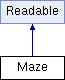
\includegraphics[height=2.000000cm]{classMaze}
\end{center}
\end{figure}
\subsection*{Public Member Functions}
\begin{DoxyCompactItemize}
\item 
\hypertarget{classMaze_a8f1cc7d8dd3fa426ace16bf32f54f24f}{
{\bfseries Maze} (int height, int width)}
\label{classMaze_a8f1cc7d8dd3fa426ace16bf32f54f24f}

\item 
\hypertarget{classMaze_a3f9b79edb99a9726da62bc6823ea9149}{
int {\bfseries get\_\-width} ()}
\label{classMaze_a3f9b79edb99a9726da62bc6823ea9149}

\item 
\hypertarget{classMaze_a43a3408e506b2f2463fc985865b3c850}{
int {\bfseries get\_\-height} ()}
\label{classMaze_a43a3408e506b2f2463fc985865b3c850}

\item 
\hypertarget{classMaze_a18724de009238efe119be4c80906416f}{
boolean {\bfseries is\_\-walkable} (int line, int column)}
\label{classMaze_a18724de009238efe119be4c80906416f}

\item 
\hypertarget{classMaze_a1156760e57f75cd36241a9244f902277}{
boolean {\bfseries is\_\-walkable} (\hyperlink{classCoord}{Coord} coord)}
\label{classMaze_a1156760e57f75cd36241a9244f902277}

\item 
\hypertarget{classMaze_ac223c8189bee28e047d4399cff5fa765}{
boolean {\bfseries is\_\-exit\_\-point} (int line, int column)}
\label{classMaze_ac223c8189bee28e047d4399cff5fa765}

\item 
\hypertarget{classMaze_a5ee98f5633093dc2e1cba6c03e4ddb54}{
boolean {\bfseries is\_\-exit\_\-point} (\hyperlink{classCoord}{Coord} coord)}
\label{classMaze_a5ee98f5633093dc2e1cba6c03e4ddb54}

\item 
\hypertarget{classMaze_a258ccfd950d62359774ed00a75591eaa}{
void {\bfseries mark\_\-solution\_\-step} (int line, int column)}
\label{classMaze_a258ccfd950d62359774ed00a75591eaa}

\item 
\hypertarget{classMaze_a0b27a912b886cd33a45d53789e4f2f1b}{
void {\bfseries mark\_\-solution\_\-step} (\hyperlink{classCoord}{Coord} coord)}
\label{classMaze_a0b27a912b886cd33a45d53789e4f2f1b}

\item 
\hypertarget{classMaze_a70725da73e2032a640bd80db1a51b1dc}{
void {\bfseries read} (Scanner scanner)}
\label{classMaze_a70725da73e2032a640bd80db1a51b1dc}

\item 
\hypertarget{classMaze_a6eb47c884e545475598f784707088f8b}{
void {\bfseries print} ()}
\label{classMaze_a6eb47c884e545475598f784707088f8b}

\end{DoxyCompactItemize}


The documentation for this class was generated from the following file:\begin{DoxyCompactItemize}
\item 
/home/marcvs/Desktop/working/pa-\/materiale/pa/codeBase/Java/src/Maze.java\end{DoxyCompactItemize}

\hypertarget{classNimGameConf}{
\section{NimGameConf Class Reference}
\label{classNimGameConf}\index{NimGameConf@{NimGameConf}}
}
\subsection*{Public Member Functions}
\begin{DoxyCompactItemize}
\item 
\hypertarget{classNimGameConf_aca38313f09d82be07a32770a9f6875cc}{
{\bfseries NimGameConf} (int n)}
\label{classNimGameConf_aca38313f09d82be07a32770a9f6875cc}

\item 
size\_\-t \hyperlink{classNimGameConf_a6562b1e5b81ef42b350abdb7b3f024be}{size} ()
\begin{DoxyCompactList}\small\item\em Functie care intoarce dimensiunea celei mai mari gramezi din joc. \end{DoxyCompactList}\item 
bool \hyperlink{classNimGameConf_a9d882cf631a20956c0e542dd71a8b726}{gameOver} ()
\begin{DoxyCompactList}\small\item\em Functie care spune daca jocul s-\/a terminat. Jocul se termina atunci cand nu mai exista nici o gramada cu cel putin trei pietricele. \end{DoxyCompactList}\item 
\hypertarget{classNimGameConf_ad8c71ec49bf1a773c169f6a57523309e}{
int \& \hyperlink{classNimGameConf_ad8c71ec49bf1a773c169f6a57523309e}{operator\mbox{[}$\,$\mbox{]}} (const unsigned int index)}
\label{classNimGameConf_ad8c71ec49bf1a773c169f6a57523309e}

\begin{DoxyCompactList}\small\item\em Operator care permite accesul la orice gramada din joc. \end{DoxyCompactList}\item 
void \hyperlink{classNimGameConf_ad19bf383bbd4eafc893491e31059d777}{split} (int heap, int a, int b)
\begin{DoxyCompactList}\small\item\em Functie care imparte o gramada in alte doua gramezi mai mici. \end{DoxyCompactList}\item 
\hypertarget{classNimGameConf_a8001a96febdfe2ce67ae8cee025a89e0}{
void \hyperlink{classNimGameConf_a8001a96febdfe2ce67ae8cee025a89e0}{unsplit} (int heap, int a, int b)}
\label{classNimGameConf_a8001a96febdfe2ce67ae8cee025a89e0}

\begin{DoxyCompactList}\small\item\em Inversul functiei split. Reasambleaza doua gramezi in gramada originala. Nu este o miscare valida de gameplay, dar poate fi utila la expandarea arborelui. \end{DoxyCompactList}\end{DoxyCompactItemize}
\subsection*{Friends}
\begin{DoxyCompactItemize}
\item 
\hypertarget{classNimGameConf_a119d80a72d6c9f144fc19036dabc1827}{
std::ostream \& {\bfseries operator$<$$<$} (std::ostream \&, const \hyperlink{classNimGameConf}{NimGameConf} \&)}
\label{classNimGameConf_a119d80a72d6c9f144fc19036dabc1827}

\end{DoxyCompactItemize}


\subsection{Member Function Documentation}
\hypertarget{classNimGameConf_a9d882cf631a20956c0e542dd71a8b726}{
\index{NimGameConf@{NimGameConf}!gameOver@{gameOver}}
\index{gameOver@{gameOver}!NimGameConf@{NimGameConf}}
\subsubsection[{gameOver}]{\setlength{\rightskip}{0pt plus 5cm}bool NimGameConf::gameOver (
\begin{DoxyParamCaption}
{}
\end{DoxyParamCaption}
)\hspace{0.3cm}{\ttfamily  \mbox{[}inline\mbox{]}}}}
\label{classNimGameConf_a9d882cf631a20956c0e542dd71a8b726}


Functie care spune daca jocul s-\/a terminat. Jocul se termina atunci cand nu mai exista nici o gramada cu cel putin trei pietricele. 

\begin{DoxyReturn}{Returns}
{\bfseries true} daca jocul s-\/a terminat, sau {\bfseries false} altfel. 
\end{DoxyReturn}
\hypertarget{classNimGameConf_a6562b1e5b81ef42b350abdb7b3f024be}{
\index{NimGameConf@{NimGameConf}!size@{size}}
\index{size@{size}!NimGameConf@{NimGameConf}}
\subsubsection[{size}]{\setlength{\rightskip}{0pt plus 5cm}size\_\-t NimGameConf::size (
\begin{DoxyParamCaption}
{}
\end{DoxyParamCaption}
)\hspace{0.3cm}{\ttfamily  \mbox{[}inline\mbox{]}}}}
\label{classNimGameConf_a6562b1e5b81ef42b350abdb7b3f024be}


Functie care intoarce dimensiunea celei mai mari gramezi din joc. 

\begin{DoxyReturn}{Returns}
Dimensiunea celei mai mari gramezi din joc (cea initiala). 
\end{DoxyReturn}
\hypertarget{classNimGameConf_ad19bf383bbd4eafc893491e31059d777}{
\index{NimGameConf@{NimGameConf}!split@{split}}
\index{split@{split}!NimGameConf@{NimGameConf}}
\subsubsection[{split}]{\setlength{\rightskip}{0pt plus 5cm}void NimGameConf::split (
\begin{DoxyParamCaption}
\item[{int}]{heap, }
\item[{int}]{a, }
\item[{int}]{b}
\end{DoxyParamCaption}
)\hspace{0.3cm}{\ttfamily  \mbox{[}inline\mbox{]}}}}
\label{classNimGameConf_ad19bf383bbd4eafc893491e31059d777}


Functie care imparte o gramada in alte doua gramezi mai mici. 


\begin{DoxyParams}{Parameters}
{\em heap} & Gramada ce trebuie impartita. \\
\hline
{\em a} & Dimensiunea primei gramezi. \\
\hline
{\em b} & Dimensiunea celei de-\/a doua gramezi. \\
\hline
\end{DoxyParams}


The documentation for this class was generated from the following file:\begin{DoxyCompactItemize}
\item 
/home/tudalex/codeBase/C++/include/Nim.h\end{DoxyCompactItemize}

\hypertarget{classRebus}{
\section{Rebus Class Reference}
\label{classRebus}\index{Rebus@{Rebus}}
}
\subsection*{Public Member Functions}
\begin{DoxyCompactItemize}
\item 
\hyperlink{classRebus_ada84d588bdfa1bd624f4a3bb27ce2c76}{Rebus} ()
\begin{DoxyCompactList}\small\item\em Constructor pentru un careu de \hyperlink{classRebus}{Rebus}. \end{DoxyCompactList}\item 
char \hyperlink{classRebus_a1da48c3c6eccfcfe78285ba3e7395bcc}{get} (unsigned int row, unsigned int column)
\begin{DoxyCompactList}\small\item\em Functie care returneaza o litera din careu. \end{DoxyCompactList}\item 
void \hyperlink{classRebus_ad6dd40d142119027fa581111509a2853}{put} (unsigned int row, unsigned int column, char c)
\begin{DoxyCompactList}\small\item\em Functie care pune o litera in careu. Functia nu are nici un efect daca respectiva celula din careu contine '$\ast$'. Daca apelul este unul invalid (in afara careului), el nu are nici un efect. \end{DoxyCompactList}\item 
void \hyperlink{classRebus_a57b95672c0bf931f1605b18c5cbed815}{putString} (unsigned int row, unsigned int column, std::string s)
\begin{DoxyCompactList}\small\item\em Functie care pune un string orizontal in careu. Functia nu are nici un efect daca nu exista spatiu suficient. \end{DoxyCompactList}\item 
void \hyperlink{classRebus_a3b93d56e569bb72d7825ddebd6e902c9}{eraseString} (unsigned int row, unsigned int column)
\begin{DoxyCompactList}\small\item\em Functie care sterge un string orizontal din careu (pana la marginea careului sau pana la urmatorul caracter '$\ast$'. \end{DoxyCompactList}\item 
void \hyperlink{classRebus_a671d4a4355f48a1dc31d82236cbd4935}{erase} (unsigned int row, unsigned int column)
\begin{DoxyCompactList}\small\item\em Functie care sterge o litera din careu. Functia nu are nici un efect daca respectiva celula din careu contine '$\ast$'. Daca apelul este unul invalid (in afara careului), el nu are nici un efect. \end{DoxyCompactList}\item 
bool \hyperlink{classRebus_ab91bb231fa7ee3fb81dee78829f6f249}{is\_\-empty} (unsigned int row, unsigned int column)
\begin{DoxyCompactList}\small\item\em Functie care verifica daca o celula din careu este libera (trebuie sa nu fie completata si sa nu fie '$\ast$'. Daca apelul este unul invalid (in afara careului), se intoarce {\bfseries false}. \end{DoxyCompactList}\item 
bool \hyperlink{classRebus_af5a546a1f074c8ed3dd744927b78a46a}{is\_\-done} ()
\begin{DoxyCompactList}\small\item\em Functie care verifica daca careul este completat valid. \end{DoxyCompactList}\end{DoxyCompactItemize}
\subsection*{Public Attributes}
\begin{DoxyCompactItemize}
\item 
\hypertarget{classRebus_a9365915f372e9f478fe5189c718f043f}{
unsigned int {\bfseries rows}}
\label{classRebus_a9365915f372e9f478fe5189c718f043f}

\item 
\hypertarget{classRebus_a68fdfd23dd2cd59b026e51cccd361469}{
unsigned int {\bfseries columns}}
\label{classRebus_a68fdfd23dd2cd59b026e51cccd361469}

\item 
\hypertarget{classRebus_a255a59b959732937887caafc0b8998f6}{
char $\ast$$\ast$ {\bfseries m}}
\label{classRebus_a255a59b959732937887caafc0b8998f6}

\item 
\hypertarget{classRebus_a6bd4ab40680f23f0da27dd05fa3cd420}{
char $\ast$$\ast$ {\bfseries ref}}
\label{classRebus_a6bd4ab40680f23f0da27dd05fa3cd420}

\end{DoxyCompactItemize}
\subsection*{Friends}
\begin{DoxyCompactItemize}
\item 
\hypertarget{classRebus_ab9c46643bd7ddd15498ceb841e192bb9}{
std::ostream \& {\bfseries operator$<$$<$} (std::ostream \&, const \hyperlink{classRebus}{Rebus} \&)}
\label{classRebus_ab9c46643bd7ddd15498ceb841e192bb9}

\item 
\hypertarget{classRebus_ac41ce284be3691d705e361a0767eabc7}{
std::istream \& {\bfseries operator$>$$>$} (std::istream \&, \hyperlink{classRebus}{Rebus} \&)}
\label{classRebus_ac41ce284be3691d705e361a0767eabc7}

\end{DoxyCompactItemize}


\subsection{Constructor \& Destructor Documentation}
\hypertarget{classRebus_ada84d588bdfa1bd624f4a3bb27ce2c76}{
\index{Rebus@{Rebus}!Rebus@{Rebus}}
\index{Rebus@{Rebus}!Rebus@{Rebus}}
\subsubsection[{Rebus}]{\setlength{\rightskip}{0pt plus 5cm}Rebus::Rebus (
\begin{DoxyParamCaption}
{}
\end{DoxyParamCaption}
)\hspace{0.3cm}{\ttfamily  \mbox{[}inline\mbox{]}}}}
\label{classRebus_ada84d588bdfa1bd624f4a3bb27ce2c76}


Constructor pentru un careu de \hyperlink{classRebus}{Rebus}. 


\begin{DoxyParams}{Parameters}
{\em rows} & Numarul de linii ale careului. \\
\hline
{\em columns} & Numarul de coloane ale careului. \\
\hline
{\em in} & Un flux din care sa se citeasca configuratia careului. \\
\hline
\end{DoxyParams}


\subsection{Member Function Documentation}
\hypertarget{classRebus_a671d4a4355f48a1dc31d82236cbd4935}{
\index{Rebus@{Rebus}!erase@{erase}}
\index{erase@{erase}!Rebus@{Rebus}}
\subsubsection[{erase}]{\setlength{\rightskip}{0pt plus 5cm}void Rebus::erase (
\begin{DoxyParamCaption}
\item[{unsigned int}]{row, }
\item[{unsigned int}]{column}
\end{DoxyParamCaption}
)\hspace{0.3cm}{\ttfamily  \mbox{[}inline\mbox{]}}}}
\label{classRebus_a671d4a4355f48a1dc31d82236cbd4935}


Functie care sterge o litera din careu. Functia nu are nici un efect daca respectiva celula din careu contine '$\ast$'. Daca apelul este unul invalid (in afara careului), el nu are nici un efect. 


\begin{DoxyParams}{Parameters}
{\em row} & Linia din careu. \\
\hline
{\em column} & Coloana din careu. \\
\hline
\end{DoxyParams}
\hypertarget{classRebus_a3b93d56e569bb72d7825ddebd6e902c9}{
\index{Rebus@{Rebus}!eraseString@{eraseString}}
\index{eraseString@{eraseString}!Rebus@{Rebus}}
\subsubsection[{eraseString}]{\setlength{\rightskip}{0pt plus 5cm}void Rebus::eraseString (
\begin{DoxyParamCaption}
\item[{unsigned int}]{row, }
\item[{unsigned int}]{column}
\end{DoxyParamCaption}
)\hspace{0.3cm}{\ttfamily  \mbox{[}inline\mbox{]}}}}
\label{classRebus_a3b93d56e569bb72d7825ddebd6e902c9}


Functie care sterge un string orizontal din careu (pana la marginea careului sau pana la urmatorul caracter '$\ast$'. 


\begin{DoxyParams}{Parameters}
{\em row} & Linia locatiei de unde incepe stringul orizontal. \\
\hline
{\em column} & Coloana locatiei de unde incepe stringul orizontal. \\
\hline
\end{DoxyParams}
\hypertarget{classRebus_a1da48c3c6eccfcfe78285ba3e7395bcc}{
\index{Rebus@{Rebus}!get@{get}}
\index{get@{get}!Rebus@{Rebus}}
\subsubsection[{get}]{\setlength{\rightskip}{0pt plus 5cm}char Rebus::get (
\begin{DoxyParamCaption}
\item[{unsigned int}]{row, }
\item[{unsigned int}]{column}
\end{DoxyParamCaption}
)\hspace{0.3cm}{\ttfamily  \mbox{[}inline\mbox{]}}}}
\label{classRebus_a1da48c3c6eccfcfe78285ba3e7395bcc}


Functie care returneaza o litera din careu. 


\begin{DoxyParams}{Parameters}
{\em row} & Linia din careu. \\
\hline
{\em column} & Coloana din careu. \\
\hline
\end{DoxyParams}
\begin{DoxyReturn}{Returns}
Caracterul de la linia si coloana respectiva din careu. Pentru o celula de careu goala se va intoarce '\_\-', iar pentru o celula de careu blocata se va intoarce '$\ast$'. Daca apelul este unul invalid (in afara careului), se intoarce '$\backslash$0'. 
\end{DoxyReturn}
\hypertarget{classRebus_af5a546a1f074c8ed3dd744927b78a46a}{
\index{Rebus@{Rebus}!is\_\-done@{is\_\-done}}
\index{is\_\-done@{is\_\-done}!Rebus@{Rebus}}
\subsubsection[{is\_\-done}]{\setlength{\rightskip}{0pt plus 5cm}bool Rebus::is\_\-done (
\begin{DoxyParamCaption}
{}
\end{DoxyParamCaption}
)\hspace{0.3cm}{\ttfamily  \mbox{[}inline\mbox{]}}}}
\label{classRebus_af5a546a1f074c8ed3dd744927b78a46a}


Functie care verifica daca careul este completat valid. 

\begin{DoxyReturn}{Returns}
{\bfseries true} daca careul este unul valid si corect completat, sau {\bfseries false} altfel. 
\end{DoxyReturn}
\hypertarget{classRebus_ab91bb231fa7ee3fb81dee78829f6f249}{
\index{Rebus@{Rebus}!is\_\-empty@{is\_\-empty}}
\index{is\_\-empty@{is\_\-empty}!Rebus@{Rebus}}
\subsubsection[{is\_\-empty}]{\setlength{\rightskip}{0pt plus 5cm}bool Rebus::is\_\-empty (
\begin{DoxyParamCaption}
\item[{unsigned int}]{row, }
\item[{unsigned int}]{column}
\end{DoxyParamCaption}
)\hspace{0.3cm}{\ttfamily  \mbox{[}inline\mbox{]}}}}
\label{classRebus_ab91bb231fa7ee3fb81dee78829f6f249}


Functie care verifica daca o celula din careu este libera (trebuie sa nu fie completata si sa nu fie '$\ast$'. Daca apelul este unul invalid (in afara careului), se intoarce {\bfseries false}. 


\begin{DoxyParams}{Parameters}
{\em row} & Linia din careu. \\
\hline
{\em column} & Coloana din careu. \\
\hline
\end{DoxyParams}
\begin{DoxyReturn}{Returns}
{\bfseries true} daca respectiva celula este libera si {\bfseries false} in caz contrar. 
\end{DoxyReturn}
\hypertarget{classRebus_ad6dd40d142119027fa581111509a2853}{
\index{Rebus@{Rebus}!put@{put}}
\index{put@{put}!Rebus@{Rebus}}
\subsubsection[{put}]{\setlength{\rightskip}{0pt plus 5cm}void Rebus::put (
\begin{DoxyParamCaption}
\item[{unsigned int}]{row, }
\item[{unsigned int}]{column, }
\item[{char}]{c}
\end{DoxyParamCaption}
)\hspace{0.3cm}{\ttfamily  \mbox{[}inline\mbox{]}}}}
\label{classRebus_ad6dd40d142119027fa581111509a2853}


Functie care pune o litera in careu. Functia nu are nici un efect daca respectiva celula din careu contine '$\ast$'. Daca apelul este unul invalid (in afara careului), el nu are nici un efect. 


\begin{DoxyParams}{Parameters}
{\em row} & Linia din careu. \\
\hline
{\em column} & Coloana din careu. \\
\hline
{\em c} & Caracterul care va fi scris in careu. \\
\hline
\end{DoxyParams}
\hypertarget{classRebus_a57b95672c0bf931f1605b18c5cbed815}{
\index{Rebus@{Rebus}!putString@{putString}}
\index{putString@{putString}!Rebus@{Rebus}}
\subsubsection[{putString}]{\setlength{\rightskip}{0pt plus 5cm}void Rebus::putString (
\begin{DoxyParamCaption}
\item[{unsigned int}]{row, }
\item[{unsigned int}]{column, }
\item[{std::string}]{s}
\end{DoxyParamCaption}
)\hspace{0.3cm}{\ttfamily  \mbox{[}inline\mbox{]}}}}
\label{classRebus_a57b95672c0bf931f1605b18c5cbed815}


Functie care pune un string orizontal in careu. Functia nu are nici un efect daca nu exista spatiu suficient. 


\begin{DoxyParams}{Parameters}
{\em row} & Linia din careu. \\
\hline
{\em column} & Coloana din careu. \\
\hline
{\em s} & Sttring care va fi scris in careu. \\
\hline
\end{DoxyParams}


The documentation for this class was generated from the following file:\begin{DoxyCompactItemize}
\item 
/home/tudalex/codeBase/C++/include/Rebus.h\end{DoxyCompactItemize}

\hypertarget{classSudokuBoard}{
\section{SudokuBoard Class Reference}
\label{classSudokuBoard}\index{SudokuBoard@{SudokuBoard}}
}
\subsection*{Classes}
\begin{DoxyCompactItemize}
\item 
class {\bfseries BitSet}
\end{DoxyCompactItemize}
\subsection*{Public Member Functions}
\begin{DoxyCompactItemize}
\item 
bool \hyperlink{classSudokuBoard_aa5d810273b58996f5eb00522dc04c012}{impossible} (int row, int col)
\begin{DoxyCompactList}\small\item\em Functie care spune daca pentru linia {\bfseries row} si coloana {\bfseries col} din careu nu mai avem nici o posibilitate de completare. \end{DoxyCompactList}\item 
int \hyperlink{classSudokuBoard_add88bcf66d345b2822335d92713b8714}{unique\_\-possibility} (int row, int col)
\begin{DoxyCompactList}\small\item\em Functie care verifica daca nu cumva pentru linia {\bfseries row} si coloana {\bfseries col} nu exista decat o singura metoda de completare. \end{DoxyCompactList}\item 
bool \hyperlink{classSudokuBoard_a4ae4146f3ebed70288b41adb9ee1d8ed}{allows} (int row, int col, int i)
\begin{DoxyCompactList}\small\item\em Functie care verifica daca este posibil sa se completeze valoarea {\bfseries i} la celula de coordonate {\bfseries row}, {\bfseries col} \end{DoxyCompactList}\item 
void \hyperlink{classSudokuBoard_aff759e2337f20e107ed7e70d5cd8ca41}{put} (int row, int col, int i)
\begin{DoxyCompactList}\small\item\em Functie care completeaza o valoare intr-\/o celula din careu. {\bfseries ATENTIE!} Este responsabilitatea voastra sa va asigurati ca nu suprascrieti o valoare deja pusa acolo! \end{DoxyCompactList}\item 
bool \hyperlink{classSudokuBoard_a1e4d6cac572c9f4d4a573265da99f517}{is\_\-empty} (int row, int col)
\begin{DoxyCompactList}\small\item\em Functie care verifica daca o celula din careu nu a fost completata. \end{DoxyCompactList}\item 
bool \hyperlink{classSudokuBoard_ad53cca0148ad57fdaa05f9b92000fe66}{is\_\-done} ()
\begin{DoxyCompactList}\small\item\em Functie care verifica daca un careu s-\/a terminat de completat. \end{DoxyCompactList}\end{DoxyCompactItemize}
\subsection*{Friends}
\begin{DoxyCompactItemize}
\item 
\hypertarget{classSudokuBoard_ac31711643f4d24c0e0e312d763a37d62}{
std::ostream \& \hyperlink{classSudokuBoard_ac31711643f4d24c0e0e312d763a37d62}{operator$<$$<$} (std::ostream \&out, \hyperlink{classSudokuBoard}{SudokuBoard} \&right)}
\label{classSudokuBoard_ac31711643f4d24c0e0e312d763a37d62}

\begin{DoxyCompactList}\small\item\em Operator care scrie o grila de Sudoku intr-\/un stream de iesire. \end{DoxyCompactList}\end{DoxyCompactItemize}


\subsection{Member Function Documentation}
\hypertarget{classSudokuBoard_a4ae4146f3ebed70288b41adb9ee1d8ed}{
\index{SudokuBoard@{SudokuBoard}!allows@{allows}}
\index{allows@{allows}!SudokuBoard@{SudokuBoard}}
\subsubsection[{allows}]{\setlength{\rightskip}{0pt plus 5cm}bool SudokuBoard::allows (
\begin{DoxyParamCaption}
\item[{int}]{row, }
\item[{int}]{col, }
\item[{int}]{i}
\end{DoxyParamCaption}
)\hspace{0.3cm}{\ttfamily  \mbox{[}inline\mbox{]}}}}
\label{classSudokuBoard_a4ae4146f3ebed70288b41adb9ee1d8ed}


Functie care verifica daca este posibil sa se completeze valoarea {\bfseries i} la celula de coordonate {\bfseries row}, {\bfseries col} 


\begin{DoxyParams}{Parameters}
{\em row} & Linia pentru care verificam \\
\hline
{\em col} & Coloana pentru care verificam \\
\hline
{\em i} & Valoarea despre care intrebam daca este permisibila \\
\hline
\end{DoxyParams}
\begin{DoxyReturn}{Returns}
Functia intoarce {\bfseries true} daca completarea este corecta. 
\end{DoxyReturn}
\hypertarget{classSudokuBoard_aa5d810273b58996f5eb00522dc04c012}{
\index{SudokuBoard@{SudokuBoard}!impossible@{impossible}}
\index{impossible@{impossible}!SudokuBoard@{SudokuBoard}}
\subsubsection[{impossible}]{\setlength{\rightskip}{0pt plus 5cm}bool SudokuBoard::impossible (
\begin{DoxyParamCaption}
\item[{int}]{row, }
\item[{int}]{col}
\end{DoxyParamCaption}
)\hspace{0.3cm}{\ttfamily  \mbox{[}inline\mbox{]}}}}
\label{classSudokuBoard_aa5d810273b58996f5eb00522dc04c012}


Functie care spune daca pentru linia {\bfseries row} si coloana {\bfseries col} din careu nu mai avem nici o posibilitate de completare. 


\begin{DoxyParams}{Parameters}
{\em row} & Linia pentru care verificam \\
\hline
{\em col} & Coloana pentru care verificam \\
\hline
\end{DoxyParams}
\begin{DoxyReturn}{Returns}
Functia intoarce {\bfseries true} daca este imposibil sa mai completezi celula de coordonate (row,col) 
\end{DoxyReturn}
\hypertarget{classSudokuBoard_ad53cca0148ad57fdaa05f9b92000fe66}{
\index{SudokuBoard@{SudokuBoard}!is\_\-done@{is\_\-done}}
\index{is\_\-done@{is\_\-done}!SudokuBoard@{SudokuBoard}}
\subsubsection[{is\_\-done}]{\setlength{\rightskip}{0pt plus 5cm}bool SudokuBoard::is\_\-done (
\begin{DoxyParamCaption}
{}
\end{DoxyParamCaption}
)\hspace{0.3cm}{\ttfamily  \mbox{[}inline\mbox{]}}}}
\label{classSudokuBoard_ad53cca0148ad57fdaa05f9b92000fe66}


Functie care verifica daca un careu s-\/a terminat de completat. 

\begin{DoxyReturn}{Returns}
Functia intoarce {\bfseries true} daca s-\/a terminat completarea careului. 
\end{DoxyReturn}
\hypertarget{classSudokuBoard_a1e4d6cac572c9f4d4a573265da99f517}{
\index{SudokuBoard@{SudokuBoard}!is\_\-empty@{is\_\-empty}}
\index{is\_\-empty@{is\_\-empty}!SudokuBoard@{SudokuBoard}}
\subsubsection[{is\_\-empty}]{\setlength{\rightskip}{0pt plus 5cm}bool SudokuBoard::is\_\-empty (
\begin{DoxyParamCaption}
\item[{int}]{row, }
\item[{int}]{col}
\end{DoxyParamCaption}
)\hspace{0.3cm}{\ttfamily  \mbox{[}inline\mbox{]}}}}
\label{classSudokuBoard_a1e4d6cac572c9f4d4a573265da99f517}


Functie care verifica daca o celula din careu nu a fost completata. 

\begin{DoxyReturn}{Returns}
Functia intoarce {\bfseries true} daca celula respectiva este libera si {\bfseries false} altfel. 
\end{DoxyReturn}
\hypertarget{classSudokuBoard_aff759e2337f20e107ed7e70d5cd8ca41}{
\index{SudokuBoard@{SudokuBoard}!put@{put}}
\index{put@{put}!SudokuBoard@{SudokuBoard}}
\subsubsection[{put}]{\setlength{\rightskip}{0pt plus 5cm}void SudokuBoard::put (
\begin{DoxyParamCaption}
\item[{int}]{row, }
\item[{int}]{col, }
\item[{int}]{i}
\end{DoxyParamCaption}
)\hspace{0.3cm}{\ttfamily  \mbox{[}inline\mbox{]}}}}
\label{classSudokuBoard_aff759e2337f20e107ed7e70d5cd8ca41}


Functie care completeaza o valoare intr-\/o celula din careu. {\bfseries ATENTIE!} Este responsabilitatea voastra sa va asigurati ca nu suprascrieti o valoare deja pusa acolo! 


\begin{DoxyParams}{Parameters}
{\em row} & Linia pentru care verificam \\
\hline
{\em col} & Coloana pentru care verificam \\
\hline
{\em i} & Valoarea pe care dorim sa o trecem in celula \\
\hline
\end{DoxyParams}
\hypertarget{classSudokuBoard_add88bcf66d345b2822335d92713b8714}{
\index{SudokuBoard@{SudokuBoard}!unique\_\-possibility@{unique\_\-possibility}}
\index{unique\_\-possibility@{unique\_\-possibility}!SudokuBoard@{SudokuBoard}}
\subsubsection[{unique\_\-possibility}]{\setlength{\rightskip}{0pt plus 5cm}int SudokuBoard::unique\_\-possibility (
\begin{DoxyParamCaption}
\item[{int}]{row, }
\item[{int}]{col}
\end{DoxyParamCaption}
)\hspace{0.3cm}{\ttfamily  \mbox{[}inline\mbox{]}}}}
\label{classSudokuBoard_add88bcf66d345b2822335d92713b8714}


Functie care verifica daca nu cumva pentru linia {\bfseries row} si coloana {\bfseries col} nu exista decat o singura metoda de completare. 


\begin{DoxyParams}{Parameters}
{\em row} & Linia pentru care verificam \\
\hline
{\em col} & Coloana pentru care verificam \\
\hline
\end{DoxyParams}
\begin{DoxyReturn}{Returns}
Functia intoarce o cifra nenula intre 1 si 9 daca exista o singura varianta de completare, si 0 daca exista mai multe variante sau nici o varianta. 
\end{DoxyReturn}


The documentation for this class was generated from the following files:\begin{DoxyCompactItemize}
\item 
/home/tudalex/codeBase/C++/include/SudokuBoard.h\item 
/home/tudalex/codeBase/C++/src/SudokuBoard.cpp\end{DoxyCompactItemize}

\hypertarget{classXOBoard}{
\section{XOBoard Class Reference}
\label{classXOBoard}\index{XOBoard@{XOBoard}}
}
\subsection*{Public Member Functions}
\begin{DoxyCompactItemize}
\item 
\hypertarget{classXOBoard_a5740df9f6637e64adb7745228820b608}{
\hyperlink{classXOBoard_a5740df9f6637e64adb7745228820b608}{XOBoard} ()}
\label{classXOBoard_a5740df9f6637e64adb7745228820b608}

\begin{DoxyCompactList}\small\item\em Constructor fara parametri care instantiaza o tabla goala pe care nu este marcat nimic. \item\end{DoxyCompactList}\item 
\hypertarget{classXOBoard_a9cc0ccf792149ff4d2fb30f159b4331d}{
{\bfseries XOBoard} (int movesX, int movesO, int moves)}
\label{classXOBoard_a9cc0ccf792149ff4d2fb30f159b4331d}

\item 
boolean \hyperlink{classXOBoard_a6c374e5e5961b1223e08df188c276379}{is\_\-empty} (int x, int y)
\begin{DoxyCompactList}\small\item\em Metoda care verifica daca o celula este libera sau nu. \item\end{DoxyCompactList}\item 
char \hyperlink{classXOBoard_a45c7e3b053887aed0d4fbaf27bad4789}{get} (int x, int y)
\begin{DoxyCompactList}\small\item\em Metoda care intoarce caracterul de pe tabla. \item\end{DoxyCompactList}\item 
void \hyperlink{classXOBoard_a21c932338885c299354e4f702a632dae}{put} (XOPlayer player, int x, int y)
\begin{DoxyCompactList}\small\item\em Metoda care bifeaza o celula de pe tabla in numele unui jucator. \item\end{DoxyCompactList}\item 
void \hyperlink{classXOBoard_a6e72af673a48b7a4de79d7b738a690c1}{erase} (int x, int y)
\begin{DoxyCompactList}\small\item\em Metoda care sterge valoarea dintr-\/o celula de pe tabla. \item\end{DoxyCompactList}\item 
boolean \hyperlink{classXOBoard_aabd4973f2aec517e4a260834170c8fe5}{is\_\-full} ()
\begin{DoxyCompactList}\small\item\em Metoda care spune daca tabla s-\/a terminat de completat sau nu. \item\end{DoxyCompactList}\item 
int \hyperlink{classXOBoard_ac7efc6b2b81c1ad846984a887394fbbc}{get\_\-score} (XOPlayer player)
\begin{DoxyCompactList}\small\item\em Metoda care intoarce scorul tablei din perspectiva jucatorului dat ca parametru. \item\end{DoxyCompactList}\item 
boolean \hyperlink{classXOBoard_a7bf161fef927f1271ccaa018b2fc8d10}{game\_\-over} ()
\begin{DoxyCompactList}\small\item\em Metoda care spune daca jocul s-\/a terminat. \item\end{DoxyCompactList}\item 
\hypertarget{classXOBoard_a1d963dd14185fa970577f23e5559f6a0}{
void {\bfseries print} ()}
\label{classXOBoard_a1d963dd14185fa970577f23e5559f6a0}

\item 
\hypertarget{classXOBoard_a5d4d4e134e7785da5ce31bddc01e9049}{
\hyperlink{classXOBoard}{XOBoard} {\bfseries clone} ()  throws CloneNotSupportedException        }
\label{classXOBoard_a5d4d4e134e7785da5ce31bddc01e9049}

\item 
\hypertarget{classXOBoard_ae3b9fec9bd85693f35a2c9c3713682e2}{
\hyperlink{classXOBoard}{XOBoard} {\bfseries tryClone} ()}
\label{classXOBoard_ae3b9fec9bd85693f35a2c9c3713682e2}

\end{DoxyCompactItemize}


\subsection{Member Function Documentation}
\hypertarget{classXOBoard_a6e72af673a48b7a4de79d7b738a690c1}{
\index{XOBoard@{XOBoard}!erase@{erase}}
\index{erase@{erase}!XOBoard@{XOBoard}}
\subsubsection[{erase}]{\setlength{\rightskip}{0pt plus 5cm}void XOBoard::erase (
\begin{DoxyParamCaption}
\item[{int}]{ x, }
\item[{int}]{ y}
\end{DoxyParamCaption}
)\hspace{0.3cm}{\ttfamily  \mbox{[}inline\mbox{]}}}}
\label{classXOBoard_a6e72af673a48b7a4de79d7b738a690c1}


Metoda care sterge valoarea dintr-\/o celula de pe tabla. 


\begin{DoxyParams}{Parameters}
\item[{\em x}]Linia X de pe tabla (intre 0 si 2) \item[{\em y}]Linia Y de pe tabla (intre 0 si 2) \end{DoxyParams}
\hypertarget{classXOBoard_a7bf161fef927f1271ccaa018b2fc8d10}{
\index{XOBoard@{XOBoard}!game\_\-over@{game\_\-over}}
\index{game\_\-over@{game\_\-over}!XOBoard@{XOBoard}}
\subsubsection[{game\_\-over}]{\setlength{\rightskip}{0pt plus 5cm}boolean XOBoard::game\_\-over (
\begin{DoxyParamCaption}
{}
\end{DoxyParamCaption}
)\hspace{0.3cm}{\ttfamily  \mbox{[}inline\mbox{]}}}}
\label{classXOBoard_a7bf161fef927f1271ccaa018b2fc8d10}


Metoda care spune daca jocul s-\/a terminat. 

\begin{DoxyReturn}{Returns}
Functia intoarce {\bfseries true} daca jocul s-\/a terminat sau {\bfseries false} daca se poate juca in continuare. 
\end{DoxyReturn}
\hypertarget{classXOBoard_a45c7e3b053887aed0d4fbaf27bad4789}{
\index{XOBoard@{XOBoard}!get@{get}}
\index{get@{get}!XOBoard@{XOBoard}}
\subsubsection[{get}]{\setlength{\rightskip}{0pt plus 5cm}char XOBoard::get (
\begin{DoxyParamCaption}
\item[{int}]{ x, }
\item[{int}]{ y}
\end{DoxyParamCaption}
)\hspace{0.3cm}{\ttfamily  \mbox{[}inline\mbox{]}}}}
\label{classXOBoard_a45c7e3b053887aed0d4fbaf27bad4789}


Metoda care intoarce caracterul de pe tabla. 


\begin{DoxyParams}{Parameters}
\item[{\em x}]Linia X de pe tabla (intre 0 si 2) \item[{\em y}]Linia Y de pe tabla (intre 0 si 2) \end{DoxyParams}
\begin{DoxyReturn}{Returns}
Dupa caz, intoarce 'X', {\bfseries 'O'} sau {\bfseries '\_\-'} 
\end{DoxyReturn}
\hypertarget{classXOBoard_ac7efc6b2b81c1ad846984a887394fbbc}{
\index{XOBoard@{XOBoard}!get\_\-score@{get\_\-score}}
\index{get\_\-score@{get\_\-score}!XOBoard@{XOBoard}}
\subsubsection[{get\_\-score}]{\setlength{\rightskip}{0pt plus 5cm}int XOBoard::get\_\-score (
\begin{DoxyParamCaption}
\item[{XOPlayer}]{ player}
\end{DoxyParamCaption}
)\hspace{0.3cm}{\ttfamily  \mbox{[}inline\mbox{]}}}}
\label{classXOBoard_ac7efc6b2b81c1ad846984a887394fbbc}


Metoda care intoarce scorul tablei din perspectiva jucatorului dat ca parametru. 


\begin{DoxyParams}{Parameters}
\item[{\em player}]Jucatorul din perspectiva caruia se calculeaza scorul. \end{DoxyParams}
\begin{DoxyReturn}{Returns}
Functia intoarce numarul de linii, coloane si diagonale complete ale jucatorului dat ca parametru. 
\end{DoxyReturn}
\hypertarget{classXOBoard_a6c374e5e5961b1223e08df188c276379}{
\index{XOBoard@{XOBoard}!is\_\-empty@{is\_\-empty}}
\index{is\_\-empty@{is\_\-empty}!XOBoard@{XOBoard}}
\subsubsection[{is\_\-empty}]{\setlength{\rightskip}{0pt plus 5cm}boolean XOBoard::is\_\-empty (
\begin{DoxyParamCaption}
\item[{int}]{ x, }
\item[{int}]{ y}
\end{DoxyParamCaption}
)\hspace{0.3cm}{\ttfamily  \mbox{[}inline\mbox{]}}}}
\label{classXOBoard_a6c374e5e5961b1223e08df188c276379}


Metoda care verifica daca o celula este libera sau nu. 


\begin{DoxyParams}{Parameters}
\item[{\em x}]Linia X de pe tabla (intre 0 si 2) \item[{\em y}]Coloana Y de pe tabla (intre 0 si 2) \end{DoxyParams}
\begin{DoxyReturn}{Returns}
Functia intoarce {\bfseries true} daca celula este libera sau {\bfseries false} daca celula este completata. 
\end{DoxyReturn}
\hypertarget{classXOBoard_aabd4973f2aec517e4a260834170c8fe5}{
\index{XOBoard@{XOBoard}!is\_\-full@{is\_\-full}}
\index{is\_\-full@{is\_\-full}!XOBoard@{XOBoard}}
\subsubsection[{is\_\-full}]{\setlength{\rightskip}{0pt plus 5cm}boolean XOBoard::is\_\-full (
\begin{DoxyParamCaption}
{}
\end{DoxyParamCaption}
)\hspace{0.3cm}{\ttfamily  \mbox{[}inline\mbox{]}}}}
\label{classXOBoard_aabd4973f2aec517e4a260834170c8fe5}


Metoda care spune daca tabla s-\/a terminat de completat sau nu. 

\begin{DoxyReturn}{Returns}
Functia intoarce {\bfseries true} daca tabla este completata la maxim sau {\bfseries false} altfel. 
\end{DoxyReturn}
\hypertarget{classXOBoard_a21c932338885c299354e4f702a632dae}{
\index{XOBoard@{XOBoard}!put@{put}}
\index{put@{put}!XOBoard@{XOBoard}}
\subsubsection[{put}]{\setlength{\rightskip}{0pt plus 5cm}void XOBoard::put (
\begin{DoxyParamCaption}
\item[{XOPlayer}]{ player, }
\item[{int}]{ x, }
\item[{int}]{ y}
\end{DoxyParamCaption}
)\hspace{0.3cm}{\ttfamily  \mbox{[}inline\mbox{]}}}}
\label{classXOBoard_a21c932338885c299354e4f702a632dae}


Metoda care bifeaza o celula de pe tabla in numele unui jucator. 


\begin{DoxyParams}{Parameters}
\item[{\em player}]Jucatorul in numele caruia se bifeaza (valori constante din clasa \hyperlink{classXOBoard}{XOBoard}) \item[{\em x}]Linia X de pe tabla (intre 0 si 2) \item[{\em y}]Linia Y de pe tabla (intre 0 si 2) \end{DoxyParams}


The documentation for this class was generated from the following file:\begin{DoxyCompactItemize}
\item 
/home/marcvs/Desktop/working/pa-\/materiale/pa/codeBase/Java/src/XOBoard.java\end{DoxyCompactItemize}

\hypertarget{classXOGame}{
\section{XOGame Class Reference}
\label{classXOGame}\index{XOGame@{XOGame}}
}
\subsection*{Public Member Functions}
\begin{DoxyCompactItemize}
\item 
\hyperlink{classXOGame_ae03433c323f4c08cfff2c9e8d26e7530}{XOGame} (ComputerAI computerAI)
\begin{DoxyCompactList}\small\item\em Constructor care instantiaza un joc in care AI-\/ul calculatorului gandeste folosindu-\/se de functia data ca parametru. \end{DoxyCompactList}\item 
\hypertarget{classXOGame_aacde44d6398b72595008996a7ac3d72d}{
void \hyperlink{classXOGame_aacde44d6398b72595008996a7ac3d72d}{humanVScomputer} ()}
\label{classXOGame_aacde44d6398b72595008996a7ac3d72d}

\begin{DoxyCompactList}\small\item\em Lanseaza in executie un joc intre un om si un calculator. Omul muta primul. \end{DoxyCompactList}\item 
\hypertarget{classXOGame_a322eaf2fceb6d4ff6f88102708b7d8ea}{
void \hyperlink{classXOGame_a322eaf2fceb6d4ff6f88102708b7d8ea}{computerVShuman} ()}
\label{classXOGame_a322eaf2fceb6d4ff6f88102708b7d8ea}

\begin{DoxyCompactList}\small\item\em Lanseaza in executie un joc intre un calculator si un om. Calculatorul muta primul. \end{DoxyCompactList}\item 
\hypertarget{classXOGame_aeb2ca697dff9b16d8abfc438e019c167}{
void \hyperlink{classXOGame_aeb2ca697dff9b16d8abfc438e019c167}{humanVShuman} ()}
\label{classXOGame_aeb2ca697dff9b16d8abfc438e019c167}

\begin{DoxyCompactList}\small\item\em Lanseaza in executie un joc intre doi oameni. \end{DoxyCompactList}\item 
\hypertarget{classXOGame_a2546fa6a5ee36ab0d380fe2b5ea5096f}{
void \hyperlink{classXOGame_a2546fa6a5ee36ab0d380fe2b5ea5096f}{computerVScomputer} ()}
\label{classXOGame_a2546fa6a5ee36ab0d380fe2b5ea5096f}

\begin{DoxyCompactList}\small\item\em Lanseaza in executie un joc intre doua calculatoare. Amandoua gandesc cu acelasi AI. Trebuie sa obtineti mereu remiza daca ati implementat optim si exhaustiv. \end{DoxyCompactList}\end{DoxyCompactItemize}


\subsection{Constructor \& Destructor Documentation}
\hypertarget{classXOGame_ae03433c323f4c08cfff2c9e8d26e7530}{
\index{XOGame@{XOGame}!XOGame@{XOGame}}
\index{XOGame@{XOGame}!XOGame@{XOGame}}
\subsubsection[{XOGame}]{\setlength{\rightskip}{0pt plus 5cm}XOGame::XOGame (
\begin{DoxyParamCaption}
\item[{ComputerAI}]{computerAI}
\end{DoxyParamCaption}
)\hspace{0.3cm}{\ttfamily  \mbox{[}inline\mbox{]}}}}
\label{classXOGame_ae03433c323f4c08cfff2c9e8d26e7530}


Constructor care instantiaza un joc in care AI-\/ul calculatorului gandeste folosindu-\/se de functia data ca parametru. 


\begin{DoxyParams}{Parameters}
{\em computerAI} & Functia pe care o va apela engine-\/ul de joc cand pune calculatorul sa gandeasca. {\bfseries $<$u$>$TREBUIE$<$/u$>$} sa respecte urmatoarea semnatura: \hyperlink{classXOBoard}{XOBoard} ComputerAI(XOBoard::Player, XOBoard). Functia data ca parametru poate fi si {\bfseries NULL}, dar in acest caz nu veti putea sa porniti jocul decat folosind metoda {\bfseries \hyperlink{classXOGame_aeb2ca697dff9b16d8abfc438e019c167}{humanVShuman()}}. \\
\hline
\end{DoxyParams}


The documentation for this class was generated from the following files:\begin{DoxyCompactItemize}
\item 
/home/tudalex/codeBase/C++/include/XOBoard.h\item 
/home/tudalex/codeBase/C++/src/XOBoard.cpp\end{DoxyCompactItemize}

\printindex
\end{document}
